\documentclass[10pt]{beamer}
\usepackage[utf8]{inputenc}
\usepackage[T1]{fontenc}
\usepackage{tikz}
\usepackage{physics}
\usepackage{mathtools}
\usepackage{csquotes}
\usepackage{tikz}
\usepackage{quantikz}
\usepackage{amsmath}
\usepackage{quantikz}
\usepackage{graphicx}
\usepackage{siunitx}
\usepackage{stmaryrd}


%\tikzcdset{every matrix/.style={ampersand replacement=\&}}

\usetheme{metropolis}

\makeatletter
\DeclareRobustCommand{\rvdots}{%
  \vbox{
    \baselineskip4\p@\lineskiplimit\z@
    \kern-\p@
    \hbox{.}\hbox{.}\hbox{.}
  }}
\makeatother

\newcommand{\defeq}{\vcentcolon=}
\newcommand{\sep}{\ensuremath{.\,}}
\definecolor{zx_red}{RGB}{232, 165, 165}
\definecolor{zx_green}{RGB}{216, 248, 216}
\definecolor{had_yellow}{RGB}{221, 218, 28}

\tikzstyle{gn}=[circle,rounded corners=0.8em,fill=zx_green,draw=black,
  line width=0.8 pt,inner sep=3pt,minimum width=1.5em,minimum height=1.5em]
\tikzstyle{rn}=[circle,rounded corners=0.8em,fill=zx_red,draw=black,
  line width=0.8 pt,inner sep=3pt,minimum width=1.5em,minimum height=1.5em]
\tikzstyle{had}=[rectangle,fill=had_yellow,draw=black,
  line width=0.8 pt,inner sep=3pt,minimum width=1.5em,minimum height=1.5em]
\tikzstyle{none}=[]
\usepackage{appendixnumberbeamer}

\usepackage{booktabs}
\usepackage[scale=2]{ccicons}

\usepackage{pgfplots}
\usepgfplotslibrary{dateplot}

\usepackage{xspace}
\newcommand{\themename}{\textbf{\textsc{metropolis}}\xspace}

\title{ZX-račun}
\subtitle{Nov pristop h kvantnem računalništvu}
\date{17.8.2022}
\author{Tadej Petrič}
\institute{Fakulteta za matematiko in fiziko}
% prednosti kvantnega računalništva vs klasično
% kvantna mehanika
% klasično kvantno rač
% 4+ zx
\begin{document}
\begin{frame}
  \maketitle
\end{frame}
\begin{frame}
  \frametitle{Definicija pajkov}
  Pajku Z z \(n\) vhodi in \(m\) izhodi pripada preslikava
  \begin{align*}
    \ket{0}^{\otimes m} \bra{0}^{\otimes n} + e^{i\alpha}\ket{1}^{\otimes m} \bra{1}^{\otimes n}.
\end{align*}
Pajku X z \(n\) vhodi in \(m\) izhodi pripada preslikava
\begin{align*}
  \ket{+}^{\otimes m} \bra{+}^{\otimes n} + e^{i\alpha}\ket{-}^{\otimes m} \bra{-}^{\otimes n}.
\end{align*}
Dodamo še kompozicijo in tenzorski produkt.
\end{frame}
\begin{frame}
  \frametitle{Inverz korena}
  \begin{align*}
    \bra{000} = \begin{bmatrix}
        1&0&0&0& 0&0&0&0
    \end{bmatrix}\\
    \bra{111} = \begin{bmatrix}
        0&0&0&0& 0&0&0&1
    \end{bmatrix}\\
    \bra{+++} = \frac{1}{2\sqrt{2}}\begin{bmatrix}
        1&1&1&1& 1&1&1&1
    \end{bmatrix}\\
    \bra{---} = \frac{1}{2\sqrt{2}} \begin{bmatrix}
        1&-1&-1&1& -1&1&1&-1
    \end{bmatrix}
\end{align*}
\end{frame}
\begin{frame}
  \frametitle{identiteta}
  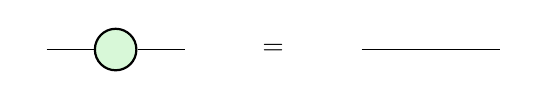
\begin{tikzpicture}
    \node (1) at (0,0) {};
    \node[style=gn] (gn) at (1,0) {};
    \node (2) at (2,0) {};
    \node (eq) at (3,0) {\(=\)};
    \node (4) at (4,0) {};
    \node (5) at (6,0) {};
    \draw (1) to (gn) to (2); 
    \draw (4) to (5);
\end{tikzpicture}
\end{frame}
\begin{frame}
  \frametitle{Združitev pajkov}
  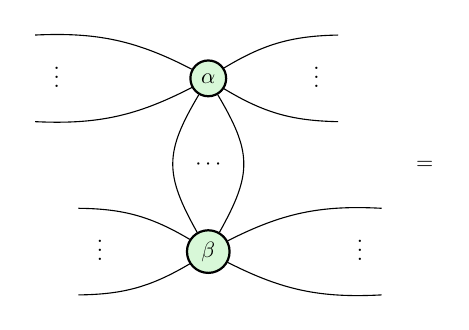
\begin{tikzpicture}[scale=0.55, every node/.style={scale=0.8}]
    \node [style=gn] (0) at (0, 2) {\(\alpha\)};
    \node [style=gn] (1) at (0, -2) {\(\beta\)};
    \node [style=none] (2) at (4, -1) {};
    \node [style=none] (3) at (4, -3) {};
    \node [style=none] (4) at (-4, 3) {};
    \node [style=none] (5) at (-4, 1) {};
    \node [style=none] (6) at (3, 3) {};
    \node [style=none] (7) at (3, 1) {};
    \node [style=none] (8) at (-3, -1) {};
    \node [style=none] (9) at (-3, -3) {};
    \node [style=none] (10) at (2.5, 2) {\(\rvdots\)};
    \node [style=none] (12) at (-2.5, -2) {\(\rvdots\)};
    \node [style=none] (13) at (3.5, -2) {\(\rvdots\)};
    \node [style=none] (14) at (0, 0) {\(\cdots\)};
    \node [style=none] (15) at (-3.5, 2) {\(\rvdots\)};
    \node [style=none] (eq) at (5, 0) {\(=\)};
    \draw [bend left=15] (4.center) to (0);
    \draw [bend right=15] (5.center) to (0);
    \draw [bend right=15] (2.center) to (1);
    \draw [bend left=15] (3.center) to (1);
    \draw [bend right, looseness=1.25] (0) to (1);
    \draw [bend left, looseness=1.25] (0) to (1);
    \draw [bend left=15] (0) to (6.center);
    \draw [bend right=15] (0) to (7.center);
    \draw [bend left=15] (8.center) to (1);
    \draw [bend right=15] (9.center) to (1);
\end{tikzpicture}
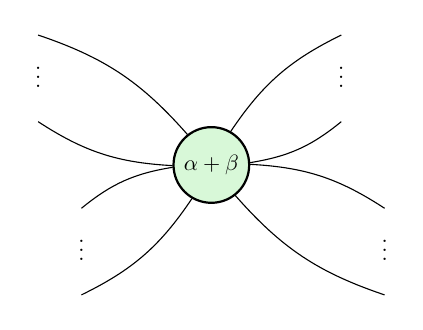
\begin{tikzpicture}[scale=0.55, every node/.style={scale=0.8}]
  \node [style=gn] (0) at (0, 0) {\(\alpha+\beta\)};
  \node [style=none] (1) at (-4, 3) {};
  \node [style=none] (2) at (-4, 1) {};
  \node [style=none] (3) at (-3, -1) {};
  \node [style=none] (4) at (-3, -3) {};
  \node [style=none] (5) at (4, -1) {};
  \node [style=none] (6) at (4, -3) {};
  \node [style=none] (7) at (3, 3) {};
  \node [style=none] (8) at (3, 1) {};
  \node [style=none] (9) at (-4, 2) {\(\rvdots\)};
  \node [style=none] (10) at (-3, -2) {\(\rvdots\)};
  \node [style=none] (11) at (3, 2) {\(\rvdots\)};
  \node [style=none] (12) at (4, -2) {\(\rvdots\)};
  \draw [bend left=15] (1.center) to (0);
  \draw [bend right=15] (2.center) to (0);
  \draw [bend left=15] (3.center) to (0);
  \draw [bend right=15] (4.center) to (0);
  \draw [bend right=15] (7.center) to (0);
  \draw [bend left=15] (8.center) to (0);
  \draw [bend right=15] (5.center) to (0);
  \draw [bend left=15] (6.center) to (0);
\end{tikzpicture}
\end{frame}
\begin{frame}
  \frametitle{Izničenje pajkov}
  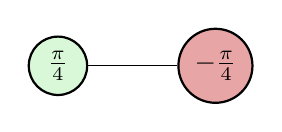
\begin{tikzpicture}
		\node [style=rn] (0) at (2, 0) {\(-\frac\pi4\)};
		\node [style=gn] (1) at (0,0) {\(\frac\pi4\)};
		\draw (0) to (1);
\end{tikzpicture}

je ekvivalentno praznemu diagramu.
\end{frame}
\begin{frame}
  \frametitle{Bialgebra}
  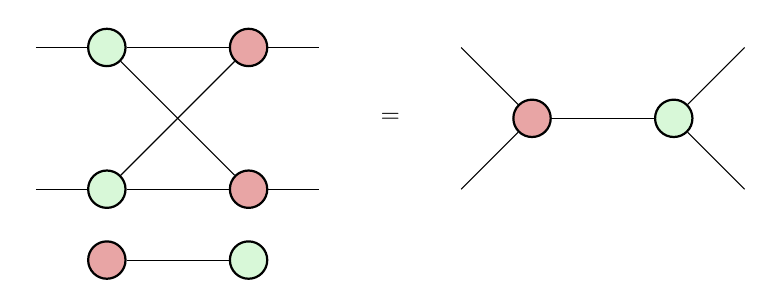
\begin{tikzpicture}[scale=0.9, every node/.style={scale=0.9}]
    \node [style=gn] (0) at (-3, 0) {};
    \node [style=gn] (1) at (-3, 2) {};
    \node [style=gn] (2) at (-1, -1) {};
    \node [style=rn] (3) at (-3, -1) {};
    \node [style=rn] (4) at (-1, 0) {};
    \node [style=rn] (5) at (-1, 2) {};
    \node [style=none] (6) at (-4, 0) {};
    \node [style=none] (7) at (-4, 2) {};
    \node [style=none] (8) at (0, 0) {};
    \node [style=none] (9) at (0, 2) {};
    \node [style=none] (10) at (1, 1) {\(=\)};
    \node [style=rn] (11) at (3, 1) {};
    \node [style=gn] (12) at (5, 1) {};
    \node [style=none] (13) at (2, 0) {};
    \node [style=none] (14) at (2, 2) {};
    \node [style=none] (15) at (6, 0) {};
    \node [style=none] (16) at (6, 2) {};
    \draw (6.center) to (0);
    \draw (7.center) to (1);
    \draw (0) to (4);
    \draw (4) to (8.center);
    \draw (1) to (5);
    \draw (5) to (9.center);
    \draw (3) to (2);
    \draw (0) to (5);
    \draw (1) to (4);
    \draw (11) to (12);
    \draw (12) to (15.center);
    \draw (12) to (16.center);
    \draw (11) to (14.center);
    \draw (11) to (13.center);
\end{tikzpicture} 
\end{frame}

\begin{frame}
  \frametitle{Pravilo kopiranja}
  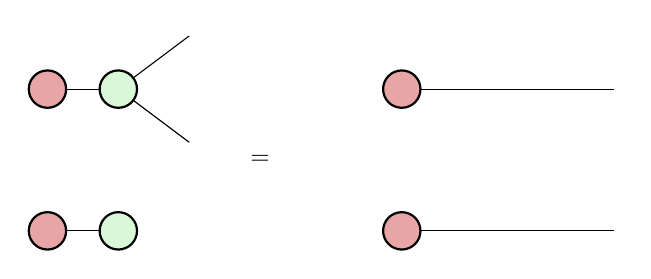
\begin{tikzpicture}[scale=0.9, every node/.style={scale=0.9}]
    \node [style=rn] (0) at (-3, -1) {};
    \node [style=rn] (1) at (-3, 1) {};
    \node [style=gn] (2) at (-2, -1) {};
    \node [style=gn] (3) at (-2, 1) {};
    \node [style=none] (4) at (-1, 0.25) {};
    \node [style=none] (5) at (-1, 1.75) {};
    \node [style=none] (7) at (0, 0) {\(=\)};
    \node [style=rn] (8) at (2, -1) {};
    \node [style=rn] (9) at (2, 1) {};
    \node [style=none] (10) at (5, -1) {};
    \node [style=none] (11) at (5, 1) {};
    \draw (0) to (2);
    \draw (1) to (3);
    \draw (3) to (4.center);
    \draw (3) to (5.center);
    \draw (8) to (10.center);
    \draw (9) to (11.center);
\end{tikzpicture}      
\end{frame}
\begin{frame}
  \frametitle{Hadamardova dekompozicija}
  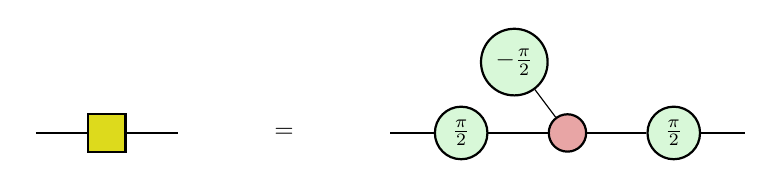
\begin{tikzpicture}[scale=0.9, every node/.style={scale=0.9}]
    \node [style=none] (0) at (-5, 0) {};
\node [style=none] (1) at (-3, 0) {};
\node [style=had] (2) at (-4, 0) {};
\node [style=none] (4) at (-1.5, 0) {\(=\)};
\node [style=none] (5) at (0, 0) {};
\node [style=none] (6) at (5, 0) {};
\node [style=rn] (7) at (2.5, 0) {};
\node [style=gn] (8) at (1, 0) {\(\frac\pi2\)};
\node [style=gn] (9) at (4, 0) {\(\frac\pi2\)};
\node [style=gn] (10) at (1.75, 1) {\(-\frac\pi2\)};
\draw (0.center) to (2);
\draw (2) to (1.center);
\draw (5.center) to (8);
\draw (8) to (7);
\draw (7) to (9);
\draw (9) to (6.center);
\draw (7) to (10);
\end{tikzpicture} 
\end{frame}
\begin{frame}
  \frametitle{Hadamardova menjava barv}
  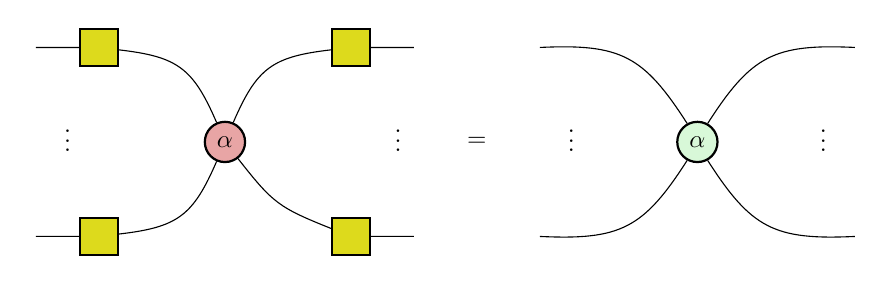
\begin{tikzpicture}[scale=0.8, every node/.style={scale=0.9}]
    \node [style=none] (0) at (-8, -1.5) {};
    \node [style=none] (1) at (-8, 1.5) {};
    \node [style=none] (2) at (-2, 1.5) {};
    \node [style=none] (3) at (-2, -1.5) {};
    \node [style=rn] (5) at (-5, 0) {\(\alpha\)};
    \node [style=had] (6) at (-7, -1.5) {};
    \node [style=had] (7) at (-7, 1.5) {};
    \node [style=had] (8) at (-3, 1.5) {};
    \node [style=had] (9) at (-3, -1.5) {};
    \node [style=none] (11) at (-1, 0) {\(=\)};
    \node [style=gn] (13) at (2.5, 0) {\(\alpha\)};
    \node [style=none] (14) at (5, 1.5) {};
    \node [style=none] (15) at (5, -1.5) {};
    \node [style=none] (16) at (0, -1.5) {};
    \node [style=none] (17) at (0, 1.5) {};
    \node [style=none] (18) at (-2.25, 0) {\(\rvdots\)};
    \node [style=none] (19) at (4.5, 0) {\(\rvdots\)};
    \node [style=none] (20) at (-7.5, 0) {\(\rvdots\)};
    \node [style=none] (21) at (0.5, 0) {\(\rvdots\)};
    \draw (0.center) to (6);
    \draw (1.center) to (7);
    \draw (8) to (2.center);
    \draw (9) to (3.center);
    \draw [bend right, looseness=1.25] (13) to (17.center);
    \draw [bend left, looseness=1.25] (13) to (16.center);
    \draw [bend right, looseness=1.25] (13) to (15.center);
    \draw [bend left, looseness=1.25] (13) to (14.center);
    \draw [bend right, looseness=1.25] (6) to (5);
    \draw [bend left, looseness=1.25] (7) to (5);
    \draw [bend left=15, looseness=1.25] (9) to (5);
    \draw [bend right, looseness=1.25] (8) to (5);
\end{tikzpicture}    
\end{frame}
\begin{frame}
  \frametitle{Eulerjevi koti}
  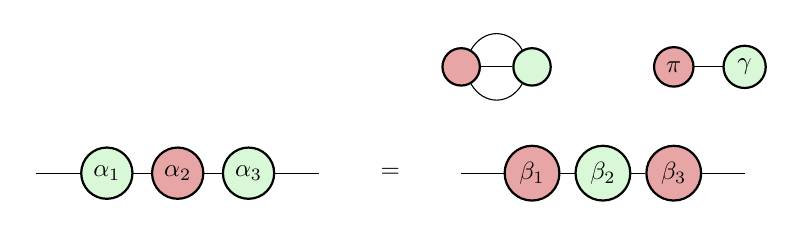
\begin{tikzpicture}[scale=0.9, every node/.style={scale=0.9}]
    \node [style=none] (0) at (-4, 0) {};
    \node [style=gn] (1) at (-3, 0) {\(\alpha_1\)};
    \node [style=gn] (2) at (-1, 0) {\(\alpha_3\)};
    \node [style=rn] (3) at (-2, 0) {\(\alpha_2\)};
    \node [style=none] (4) at (0, 0) {};
    \node [style=none] (5) at (1, 0) {\(=\)};
    \node [style=none] (6) at (2, 0) {};
    \node [style=none] (7) at (6, 0) {};
    \node [style=gn] (8) at (4, 0) {\(\beta_2\)};
    \node [style=rn] (9) at (5, 0) {\(\beta_3\)};
    \node [style=rn] (10) at (3, 0) {\(\beta_1\)};
    \node [style=rn] (11) at (2, 1.5) {};
    \node [style=gn] (12) at (3, 1.5) {};
    \node [style=rn] (13) at (5, 1.5) {\(\pi\)};
    \node [style=gn] (14) at (6, 1.5) {\(\gamma\)};
    \draw (0.center) to (1);
    \draw (1) to (3);
    \draw (3) to (2);
    \draw (2) to (4.center);
    \draw [bend left=60, looseness=1.25] (11) to (12);
    \draw [bend right=60, looseness=1.25] (11) to (12);
    \draw (11) to (12);
    \draw (13) to (14);
    \draw (6.center) to (10);
    \draw (10) to (8);
    \draw (8) to (9);
    \draw (9) to (7.center);
\end{tikzpicture}    
\end{frame}
\begin{frame}
  \frametitle{Eulerjevi koti}
  \begin{align*}
    x^+ &= \frac{\alpha_1 + \alpha_3}{2}\\
    x^- &= x^+-\alpha_3\\
    z &= \cos\left(\frac{\alpha_2}{2}\right)\cos\left(x^+\right) + i\sin\left(\frac{\alpha_2}{2}\right)\cos\left(x^-\right)\\
    z' &= \cos\left(\frac{\alpha_2}{2}\right)\sin\left(x^+\right) - i\sin\left(\frac{\alpha_2}{2}\right)\sin\left(x^-\right)\\
  \beta_1 &= \arg z + \arg z'\\
  \beta_2 &= 2\arg\left(i+\left\lvert\frac{z}{z'}\right\rvert\right)\\
  \beta_3 &= \arg z - \arg z'\\
  \gamma &= x^+-\arg z + \frac{\alpha_2-\beta_2}{2}
\end{align*}
\end{frame}

\begin{frame}
  \frametitle{Izrek: Hopfov zakon}
  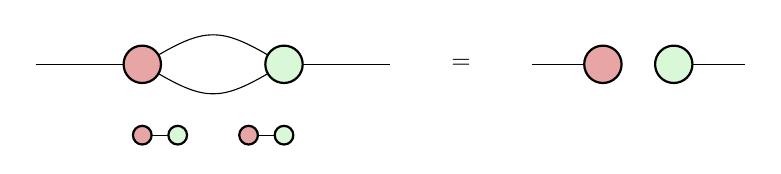
\begin{tikzpicture}[scale=0.9, every node/.style={scale=0.9}]
		\node [style=rn] (0) at (-0.5, 0) {};
		\node [style=rn, scale=0.5] (1) at (-0.5, -1) {};
		\node [style=rn, scale=0.5] (2) at (1, -1) {};
		\node [style=gn] (3) at (1.5, 0) {};
		\node [style=gn, scale=0.5] (4) at (0, -1) {};
		\node [style=gn, scale=0.5] (5) at (1.5, -1) {};
		\node [style=none] (6) at (-2, 0) {};
		\node [style=none] (7) at (3, 0) {};
		\node [style=none] (8) at (4, 0) {\(=\)};
		\node [style=none] (9) at (5, 0) {};
		\node [style=none] (10) at (8, 0) {};
		\node [style=rn] (11) at (6, 0) {};
		\node [style=gn] (12) at (7, 0) {};
		\draw [bend left, looseness=1.25] (0) to (3);
		\draw (1) to (4);
		\draw (2) to (5);
		\draw [bend right, looseness=1.25] (0) to (3);
		\draw (6.center) to (0);
		\draw (3) to (7.center);
		\draw (9.center) to (11);
		\draw (10.center) to (12);
\end{tikzpicture}
\end{frame}
\begin{frame}
  \frametitle{Kvantna teleportacija}
  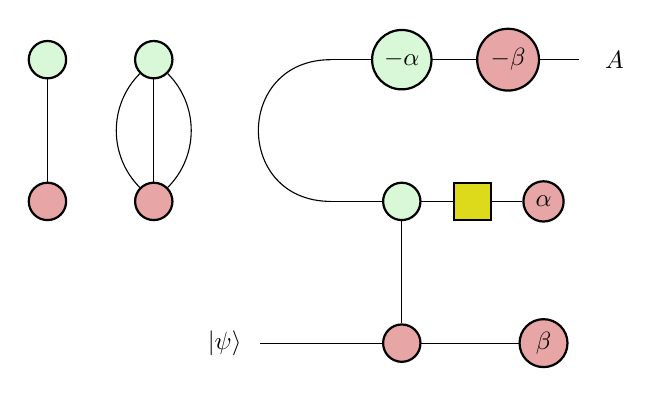
\begin{tikzpicture}[scale=0.9, every node/.style={scale=0.9}]
    \node [style=none] (1) at (1, 1) {};
    \node [style=none] (2) at (1, -1) {};
    \node [style=gn] (3) at (-1.5, 1) {};
    \node [style=rn] (4) at (-1.5, -1) {};
    \node [style=none] (5) at (-0.5, -3) {\(\ket{\psi}\)};
    \node [style=none] (7) at (5, 1) {\(A\)};
    \node [style=none] (8) at (0, -3) {};
    \node [style=gn] (9) at (2, -1) {};
    \node [style=rn] (10) at (2, -3) {};
    \node [style=had] (11) at (3, -1) {};
    \node [style=gn] (14) at (-3, 1) {};
    \node [style=rn] (15) at (-3, -1) {};
    \node [style=rn] (16) at (4, -1) {\(\alpha\)};
    \node [style=rn] (17) at (4, -3) {\(\beta\)};
    \node [style=gn] (18) at (2, 1) {\(-\alpha\)};
    \node [style=rn] (19) at (3.5, 1) {\(-\beta\)};
    \node [style=none] (20) at (4.5, 1) {};
    \draw (3) to (4);
    \draw [bend left=45] (3) to (4);
    \draw [bend right=45] (3) to (4);
    \draw [bend right=90, looseness=1.75] (1.center) to (2.center);
    \draw (2.center) to (9);
    \draw (9) to (11);
    \draw (8.center) to (10);
    \draw (9) to (10);
    \draw (14) to (15);
    \draw (11) to (16);
    \draw (10) to (17);
    \draw (1.center) to (18);
    \draw (18) to (19);
    \draw (19) to (20.center);
\end{tikzpicture} 
\end{frame}

\end{document}